\chapter{Metodología}

En este apartado describiremos la metodología llevada a cabo en el proyecto. Una metodología es un conjunto de procesos, métodos y prácticas llevadas a cabo para asegurar, en la mayor medida posible, calidad en el producto final y en el tiempo acordado.

En nuestro caso, al ser un proyecto realizado por una sola persona y con un tiempo diario limitado, hemos optado por adaptar una serie de ideas y valores principales de varias metodologías.

\section{Desarrollo en cascada}

El desarrollo en cascada, también denominado como modelo en cascada, es una metodología con varias etapas donde, para pasar a la siguiente, es completamente necesario que la anterior haya acabado y esté completada.

Las ventajas que ofrece en desarrollo en cascada es que es muy sencillo de implementar en comparación con otras metodologías, requiere menos tiempo y capital para hacerlo funcionar de manera óptima y es usado con bastante frecuencia.

La mayor desventaja es que detectar un error en una de las fases finales puede significar tener que replantear los pasos tomados en las anteriores, perdiendo parte del progreso realizado.

\subsection{Etapas del desarrollo en cascada}

\paragraph{Análisis de requisitos}: 

En esta fase se definen y determinan los requisitos que el software debe de cumplir entre el desarrollador y el cliente. Generalmente se generan documentos que formalizan dichas decisiones para no tener que cambiarlas en el futuro, dado que un cambio en los requisitos puede significar cambiar gran parte del proyecto, por lo que llegar a un consenso es necesario.

\paragraph{Diseño}: 

Una vez del análisis haya finalizado, es hora del diseño. La idea principal es descomponer lo detallado durante el análisis de requisitos con el cliente y crear diferentes diagramas y diseños que ayuden a los programadores a entender lo que debe de ser realizado y cómo debe de funcionar, incluyendo pseudocódigo o algoritmos a alto nivel en caso de que sea necesario.

\paragraph{Implementación}:

En esta fase es donde se escribe el código fuente en base a lo espeficicado anteriormente, intentando dar gran importancia a la reutilización del código siempre y cuando sea posible. También es importante tener en cuenta la creación de tests y la realización de las primeras pruebas preliminares por parte de los programadores.

\paragraph{Verificación}:

Este es el momento final en el que el cliente es capaz de probar lo desarrollado. El programa debe de estar bien testado por parte de los programadores para evitar la mayoría de los problemas que pueden ocasionarse en esta fase.

\paragraph{Mantenimiento}:

Una vez el software ha finalizado y se ha entregado al usuario final, empieza la fase de mantenimiento. En ella el usuario final pedirá que se resuelvan problemas, se añadan nuevas funcionalidades y se cambien otras ya añadidas en base a los nuevos requisitos que vayan apareciendo y no se tuvieron en cuenta en el principio. Esta es una de las fases más críticas, dado que se estima que alrededor de un 80\% de los recursos de un proyecto se emplean en el mantenimiento \footnote{\url{http://eu.wiley.com/WileyCDA/WileyTitle/productCd-0471170011.html}}.

\begin{figure}[H]
		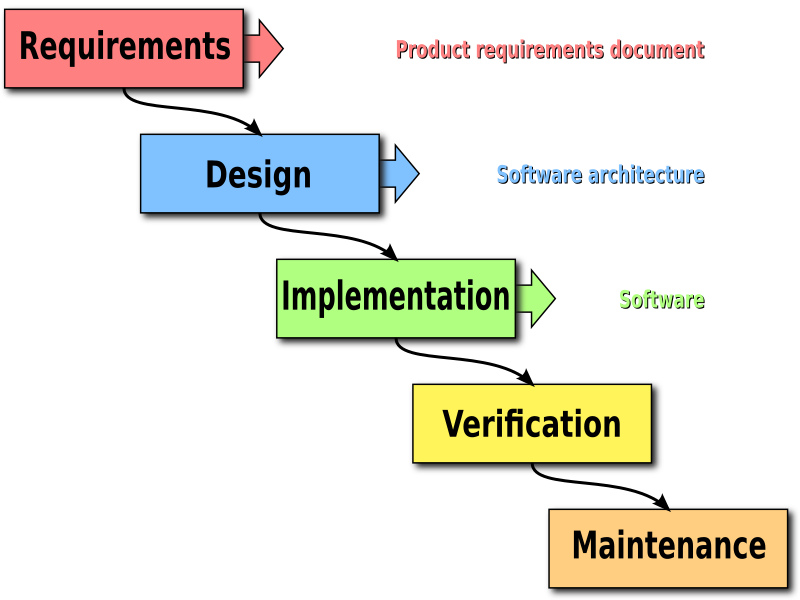
\includegraphics[width=\textwidth,height=\textheight,keepaspectratio]{./img/Waterfall_model.png}
	\caption{Estructura general de una etapa del desarrollo en cascada}
	\label{fig:cascadadesarrollo}
\end{figure}

\section{Scrum}

Scrum es una metodología ágil definida inicialmente por Hirotaka Takeuchi y Ikujiro Nonaka en 1986 \footnote{\url{https://cb.hbsp.harvard.edu/cbmp/product/86116-PDF-ENG}}. Su relativa sencillez, así como su flexibilidad y orientación al trabajo en equipo, hace que Scrum sea una de las metologías más usadas en el desarrollo de software, sobre todo en entornos laborales donde el equipo de desarrollo no es gigante (aunque su implementación también es posible en estos casos).

\subsection{Prácticas recomendadas y bases de Scrum}

Uno de los aspectos esenciales de scrum es el ``sprint'', que se trata de un bloque temporal de tiempo (generalmente de entre 2 y 4 semanas) donde el equipo de desarrollo trabajará para llegar a un objetivo determinado, generalmente acabar todas las tareas definidas para ese sprint. 
Al principio de cada sprint  el ``product owner'' y ``scrum master'' definirán las tareas que se querrán realizar en dicho sprint y que se encuentran en el backlog\footnote{Lista de tareas que se quieren realizar en el producto y que suele ir creciendo a medida que los usuarios encuentran fallos o necesitan nuevas funcionalidades. Generalmente el product owner es el encargado de organizar y decidir las tareas que tienen más prioridad}. Todos los integrantes del grupo de desarrollo, así como el propio product owner y scrum master, decidirán cuánto esfuerzo o tiempo llevará realizar cada tarea (hay algunas formas de decidir esto, como planning poker, pero no es muy relevante en nuestro caso), dividiéndola en tareas menores en caso de que sea demasiado grande. También se decidirá quién hará qué.

Durante cada día del desarrollo hay una pequeña reunión llamada ``sprint stand-up'' donde cada desarrollador comenta brevemente lo que ha hecho el día anterior, qué tiene planteado realizar ese día y si se ha encontrado con algún problema que le impida continuar.

Al acabar cada sprint, el equipo se reúne de nuevo para analizar lo que ha ido bien, qué problemas hubo y las mejoras que se tener en cuenta de cara al futuro. De esta manera, cada nuevo sprint será más preciso (dado que sabremos la cantidad de trabajo que cada desarrollador es capaz de hacer en el periodo definido de tiempo) e incluirán el ``feedback'' de los propios programadores.

Estas son las características eseciales de Scrum, pero al tratarse de una metodología ágil, nada es inamovible. Dependiendo del equipo y de las necesidades del mismo, se pueden cambiar o introducir nuevas ideas que mejoren el proceso para ese grupo de programadores en concreto.

\begin{figure}[H]
		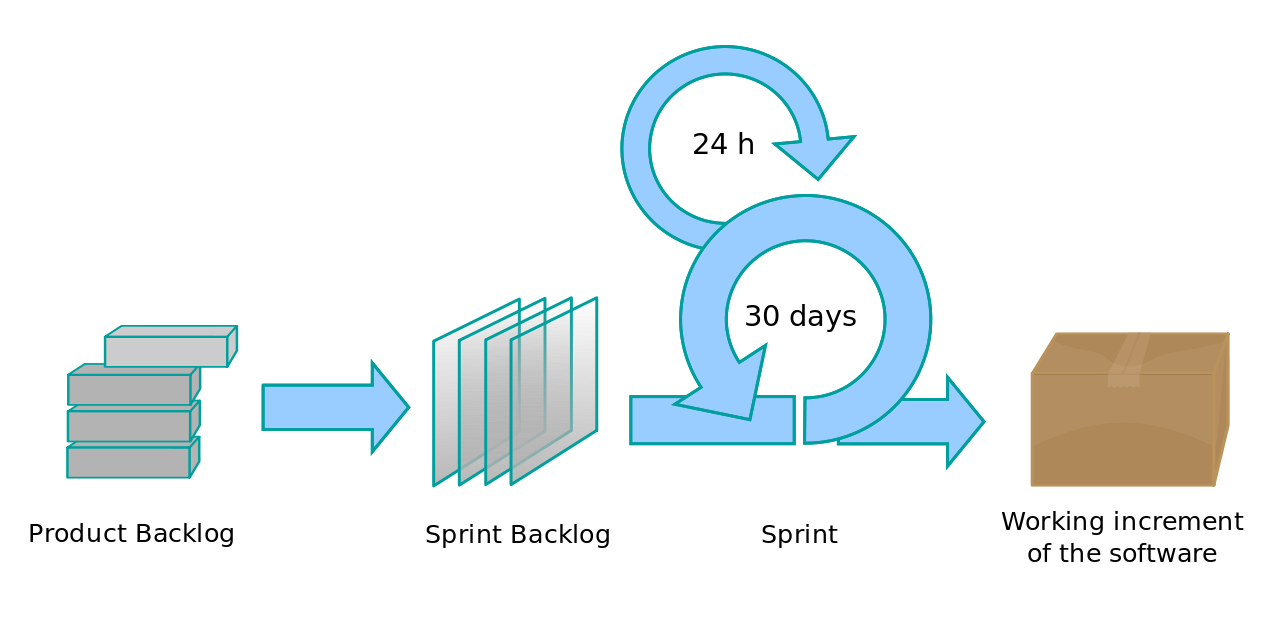
\includegraphics[width=\textwidth,height=\textheight,keepaspectratio]{./img/scrumprocess.png}
	\caption{Proceso concreto de scrum. En este caso el sprint dura 4 semanas}
	\label{fig:scrumproceso}
\end{figure}

\subsection{Valores de Scrum}

\subsubsection{Concentración}

Al tener que finalizar las tareas asignadas al final del sprint, la concentración del equipo en general y de cada uno de los miembros es esencial. Para logar este objetivo, el product owner es el encargado de responder las preguntas del resto de la compañía en nombre de los desarrolladores y solamente molestarlos en caso de que sea realmente necesario. 

\subsubsection{Coraje}

Dado que Scrum es una metodología de equipo, la ayuda entre cada uno de los miembros es algo esencial. De la misma forma, cada persona debe de ser capaz de enfrentarse a nuevos retos y asumir nuevas responsabilidades para que, en conjunto, el producto final sea el deseado. 

\subsubsection{Compromiso}

Cada integrante tiene que saber lo que puede hacer y comprometerse a ello. Una vez la reunión inicial se haya completado, es importante que cada uno sepa lo que tiene que hacer y pregunte en caso de que no tenga algo claro o crea que no puede llegar a terminar lo especificado durante la reunión. Cada programador debe de comprometerse con lo establecido para lograr el éxito del equipo.

\subsubsection{Sinceridad}

Ser capaz de asumir los errores es la clave para mejorar y evolucionar como un equipo. Si un miembro del equipo de desarrollo se queda estancado en un problema y no avisa al resto de sus compañeros, el sprint en su totalidad puede llegar a fracasar. Asumir responsabilidades, errores y pedir ayuda cuando sea necesario debe de ser una práctica habitual en Scrum.

\subsubsection{Respeto}

Similar al anterior punto. Al trabajar en equipo es imprescindible que tanto los logros como los fracasos se tomen como una nueva forma de aprender y mejorar, por lo que el respeto mutuo y asumir los errores es la mejor forma de evolucionar, tanto individualmente como en equipo.

\section{Metodología elegida}
\label{sec:metodologiaelegida}

Mayoritariamente hemos usado una metodología en cascada con algunos elementos de Scrum.

Para las características grandes del proyecto como la creación de los mapas, enemigos, sistema creación de frases, etc. nos hemos basado en cascada para analizar lo que tenemos que realizar, crear el diseño, implementarlo (empezando siempre por los tests, tal y como comentaremos a continuación) y verificarlo. Sin embargo, y dado que los juegos tienden a querer mejorarse continuamente con nuevos elementos de diferente importancia y tamaño (tanto de nuestra parte como de la gente que lo ha probado), tiene sentido mantener un backlog con todas las nuevas ideas y \textit{feedback} recogido, algo de lo que Scrum es maestro. También hemos seguido la idea de la creación de tareas cortas (de no más de 8 horas, en caso de que haya algo de mayor cantidad deberá de ser dividido en subtareas) y sprints, donde cada mes intentaremos tener un elemento del juego finalizado con varias tareas finalizadas a final de cada semana. De esta manera somos capaces de seguir más fácilmente el progreso que hemos realizado y tenemos constancia de los nuevos elementos que queremos implementar en un futuro, así como los bugs que arreglar en próximos sprints.
Al acabar con el núcleo del juego, la mayor parte de las tareas a realizar a continuación son pequeños cambios y nuevos elementos que no trastocan el diseño realizado del proyecto, por lo que seguir una metodología ágil como scrum es el mejor paso a seguir para terminar las tareas más relevantes lo antes posible.

Por último, también hemos seguido la práctica de \textit{test driven development} (desarrollo guiado por pruebas) cuya base está en, por cada nueva tarea a realizar, implementar primero los tests unitarios (que, lógicamente, fallarán) y luego programar la solución en sí para que el test sea válido, refractorizando la solución en caso de que no sea la ideal. Esto nos dará desde el primer momento una clara idea de lo que queremos hacer antes de ponernos con la implementación y nos asegurará de que siempre tendremos el test hecho.